% !TeX encoding = UTF-8 Unicode
% !TeX program = LuaLaTeX
% !TeX spellcheck = LaTeX

% Author : lzh
% Description : Convex Optimization Homework 5 Report 1

\documentclass[english]{pkupaper}

\usepackage[paper, algorithm, si]{def}

\newcommand{\cuniversity}{Peking University}
\newcommand{\cthesisname}{Convex Optimization Homework 5}
\newcommand{\titlemark}{Homework 5 Report 1}

\title{\titlemark}
\author{%
	\begin{tabular}{c}
李知含 \\
1600010653
	\end{tabular}%
}

	\begin{document}

	\maketitle

\section{Answers to questions}

\begin{thmquestion}[1]
The functions are \verb"l1_cvx_mosek" and \verb"l1_cvx_gurobi" in module \verb"l1_cvx_mosek". Note that the codes are implemented using CVXPY, which is an alternative of CVX in Python.
\end{thmquestion}

\begin{thmquestion}[2]
The model is equivalent to QP
\begin{equation}
\begin{array}{ll}
\mtx{minimize} & \frac{1}{2} y^{\rmut} y + \mu 1^{\rmut} t, \\
\mtx{subject to} & A x - y = b, \\
& -t \preceq x \preceq t,
\end{array}
\end{equation}
The functions are \verb"l1_mosek_qp" in module \verb"solver_mosek" and \verb"l1_gurobi_noexpand" in module \verb"solver_gurobi".
\end{thmquestion}

\begin{thmquestion}[3 (a)]
The model is first equivalent to QP
\begin{equation}
\begin{array}{ll}
\mtx{minimize} & \frac{1}{2} \rbr{ A x - b }^{\rmut} \rbr{ A x - b } + \mu 1^{\rmut} t, \\
\mtx{subject to } & -t \preceq x \preceq t.
\end{array}
\end{equation}
Denote $ t + x $ and $ t - x $ by $ u, v $ respectively, and this model is equivalent to
\begin{equation}
\begin{array}{ll}
\mtx{minimize} & \frac{1}{2} \rbr{ \frac{1}{2} A \rbr{ u - v } - b }^{\rmut} \rbr{ \frac{1}{2} A \rbr{ u - v } - b } + \frac{1}{2} \mu 1^{\rmut} \rbr{ u + v }, \\
\mtx{subject to} & u \succeq 0, \\
& v \succeq 0,
\end{array}
\end{equation}
which is quadratic program with box constraints.

The corresponding algorithm is shown in Algorithm \ref{Alg:ProjNaive}.

\begin{algorithm}
\SetAlgoLined

\KwData{$A$, $b$, $mu$, $x^{\rbr{0}}$, $\eta$}

$ i \slar 0 $\;
$ u^{\rbr{0}} \slar 2 \max \cbr{ x^{\rbr{0}}, 0 } $\;
$ v^{\rbr{0}} \slar 2 \min \cbr{ x^{\rbr{0}}, 0 } $\;

\While{not satisfies stop condition}
{
	$ \nabla u^{\rbr{i}} \slar \frac{1}{2} A^{\rmut} \rbr{ \frac{1}{2} A \rbr{ u^{\rbr{i}} - v^{\rbr{i}} } - b } + \frac{1}{2} \mu 1^{\rmut} $\;
	$ \nabla v^{\rbr{i}} \slar -\frac{1}{2} A^{\rmut} \rbr{ \frac{1}{2} A \rbr{ u^{\rbr{i}} - v^{\rbr{i}} } - b } + \frac{1}{2} \mu 1^{\rmut} $\;
	$ u^{\rbr{ i + 1 }} \slar u^{\rbr{i}} - \eta \nabla u^{\rbr{i}} $\;
	$ v^{\rbr{ i + 1 }} \slar v^{\rbr{i}} - \eta \nabla v^{\rbr{i}} $\;
	$ u^{\rbr{ i + 1 }} \slar \max \cbr{ u^{\rbr{ i + 1 }}, 0 } $\;
	$ v^{\rbr{ i + 1 }} \slar \max \cbr{ v^{\rbr{ i + 1 }}, 0 } $\;
	$ i \slar i + 1 $\;
}

$ x^{\rbr{i}} = \frac{1}{2} \rbr{ u^{\rbr{i}} - v^{\rbr{i}} } $\;

\caption{Projection gradient method with fixed step size} \label{Alg:ProjNaive}
\end{algorithm}

First increasing $\mu$, and then decreasing $\mu$ exponentially to the original value result in better numerical result. The algorithm is shown in Algorithm \ref{Alg:ProjExpReg}.

\begin{algorithm}
\SetAlgoLined

\KwData{$A$, $b$, $mu$, $x^{\rbr{0}}$, $\eta$, $i_0$, $k$}

$ i \slar 0 $\;
$ u^{\rbr{0}} \slar 2 \max \cbr{ x^{\rbr{0}}, 0 } $\;
$ v^{\rbr{0}} \slar 2 \min \cbr{ x^{\rbr{0}}, 0 } $\;

\While{not satisfies stop condition}
{
	$ \mu^{\rbr{i}} \slar \mu \se^{ k \max \cbr{ i_0 - i, 0 } } $\; 
	$ \nabla u^{\rbr{i}} \slar \frac{1}{2} A^{\rmut} \rbr{ \frac{1}{2} A \rbr{ u^{\rbr{i}} - v^{\rbr{i}} } - b } + \frac{1}{2} \mu^{\rbr{i}} 1^{\rmut} $\;
	$ \nabla v^{\rbr{i}} \slar -\frac{1}{2} A^{\rmut} \rbr{ \frac{1}{2} A \rbr{ u^{\rbr{i}} - v^{\rbr{i}} } - b } + \frac{1}{2} \mu^{\rbr{i}} 1^{\rmut} $\;
	$ u^{\rbr{ i + 1 }} \slar u^{\rbr{i}} - \eta \nabla u^{\rbr{i}} $\;
	$ v^{\rbr{ i + 1 }} \slar v^{\rbr{i}} - \eta \nabla v^{\rbr{i}} $\;
	$ u^{\rbr{ i + 1 }} \slar \max \cbr{ u^{\rbr{ i + 1 }}, 0 } $\;
	$ v^{\rbr{ i + 1 }} \slar \max \cbr{ v^{\rbr{ i + 1 }}, 0 } $\;
	$ i \slar i + 1 $\;
}

$ x^{\rbr{i}} = \frac{1}{2} \rbr{ u^{\rbr{i}} - v^{\rbr{i}} } $\;

\caption{Projection gradient method with fixed step size and modified $\mu$} \label{Alg:ProjExpReg}
\end{algorithm}

These two algorithms are implemented by \verb"l1_proj_grad" in module \verb"method_proj_grad".
\end{thmquestion}

\begin{thmquestion}[3 (b)]
The corresponding algorithm is shown in Algorithm \ref{Alg:SubNaive}, where the sign functions are used for sub-gradients.

\begin{algorithm}
\SetAlgoLined

\KwData{$A$, $b$, $mu$, $x^{\rbr{0}}$, $\eta$}

$ i \slar 0 $\;

\While{not satisfies stop condition}
{
	$ \nabla x^{\rbr{i}} \slar A^{\rmut} \rbr{ A x - b } + \mu \opsgn x^{\rbr{i}} $\;
	$ x^{\rbr{ i + 1 }} \slar x^{\rbr{i}} - \eta \nabla x^{\rbr{i}} $\;
	$ i \slar i + 1 $\;
}

\caption{Sub-gradient method with fixed step size} \label{Alg:SubNaive}
\end{algorithm}

The same strategy of adjusting $\mu$ here, as shown in Algorithm \label{Alg:SubExpReg}.

\begin{algorithm}
\SetAlgoLined

\KwData{$A$, $b$, $mu$, $x^{\rbr{0}}$, $\eta$, $i_0$, $k$}

$ i \slar 0 $\;

\While{not satisfies stop condition}
{
	$ \mu^{\rbr{i}} \slar \mu \se^{ k \max \cbr{ i_0 - i }, 0 } $\;
	$ \nabla x^{\rbr{i}} \slar A^{\rmut} \rbr{ A x - b } + \mu^{\rbr{i}} \opsgn x^{\rbr{i}} $\;
	$ x^{\rbr{ i + 1 }} \slar x^{\rbr{i}} - \eta \nabla x^{\rbr{i}} $\;
	$ i \slar i + 1 $\;
}

\caption{Sub-gradient method with fixed step size and modified $\mu$} \label{Alg:SubExpReg}
\end{algorithm}

These two algorithms are implemented by \verb"l1_sub_grad" in module \verb"method_sub_grad".
\end{thmquestion}

\section{Numerical results}

Numerical results are shown in Table \ref{Tbl:NumRes}.

\begin{table}[htbp]
\centering
\begin{tabular}{|c|c|c|c|c|c|}
\hline
& time (\Si{\second}) & setup time (\Si{\second}) & solve time (\Si{\second}) & variables & iterations \\ \hline
CVXPY-MOSEK & 1.088 & 0.077 & 0.620 & NA & 9  \\ \hline
CVXPY-Gurobi & 15.799 & NA & 2.783 & NA & NA \\ \hline
MOSEK & 0.785 & 0.094 & 0.681 & 2560 & 9 \\ \hline
Gurobi & 18.729 & 17.195 & 1.074 & 2560 & 14 \\ \hline
Algorithm \ref{Alg:ProjNaive} & 1.618 & NA & NA & 2048 & 2000 \\ \hline
Algorithm \ref{Alg:ProjExpReg} & 1.602 & NA & NA & 2048 & 2000 \\ \hline
Algorithm \ref{Alg:SubNaive} & 1.149 & NA & NA & 1024 & 2000 \\ \hline
Algorithm \ref{Alg:SubExpReg} & 1.142 & NA & NA & 1024 & 2000 \\ \hline
\end{tabular}

\ 

\begin{tabular}{|c|c|c|c|c|c|}
\hline
& primal objective & approximation error & error to known & error to GT \\ \hline
CVXPY-MOSEK & 7.561e-02 & 2.060e-07 & 0.000e+00 & 1.641e-05 \\ \hline
CVXPY-Gurobi & 7.561e-02 & 1.449e-07 & 1.093e-05 & 6.298e-06 \\ \hline
MOSEK & 7.561e-02 & 1.785e-07 & 6.618e-05 & 1.242e-05 \\ \hline
Gurobi & 7.561e-02 & 1.082e-07 & 1.446e-05 & 2.555e-06 \\ \hline
Algorithm \ref{Alg:ProjNaive} & 5.764e-01 & 1.041e-07 & 1.253e+00 & 1.253e+00 \\ \hline
Algorithm \ref{Alg:ProjExpReg} & 7.561e-02 & 1.081e-07 & 1.450e-05 & 2.509e-06 \\ \hline
Algorithm \ref{Alg:SubNaive} & 3.830e-01 & 2.525e-07 & 1.405e+00 & 1.405e+00 \\ \hline
Algorithm \ref{Alg:SubExpReg} & 7.561e-02 & 4.965e-07 & 1.305e-05 & 4.469e-06 \\ \hline
\end{tabular}

\caption{Numerical results} \label{Tbl:NumRes}
\end{table}

In Table \ref{Tbl:NumRes}, ``approximation error'' stands for $ \frac{1}{2} \norm{ A x - b }_2^2 $, ``error to known'' stands for the error to known solution obtained by MOSEK from CVXPY, and ``error to GT'' stands for the error to \verb"u". (Note that the optimization problem is derived from compressive sensing, which finds a sparse representation of a optimization problem. Therefore, we denotes \verb"u" to be ``ground-truth'', which is solution to be reconstructed, even if it is not the exact solution of the optimization problem)

All the codes are implemented in Python. These results are carried out on a computer with Intel Core i7-6500U (4 threads) and 7894 MiB RAM. The operating system is Arch Linux 4.13.12 64-bit and the Python environment is provided by Anaconda 4.3.30. The versions of Python, NumPy, CVXPY, MOSEK and Gurobi are 3.6.2, 1.13.1, 0.4.8, 8.1.31, 7.5.1 respectively.

In Algorithm \ref{Alg:ProjNaive}, $ \eta = 0.001 $. In Algorithm \ref{Alg:ProjExpReg}, $ \eta = 0.002 $, $ i_0 = 1500 $ and $ \mu^{\rbr{0}} = 1000 $. In Algorithm \ref{Alg:SubNaive}, $ \eta = 0.0002 $. In Algorithm \ref{Alg:SubExpReg}, $ \eta = 0.0005 $, $ i_0 = 1500 $ and $ \mu^{\rbr{0}} = 1000 $.

$x^{\rbr{0}}$ is not used when direct calling CVXPY or solvers.

\section{Interpretations and Discussions}

From the result, all algorithms except Algorithm \ref{Alg:ProjNaive} and \ref{Alg:SubNaive} converges to the optimal solution.

The intuition of modifications in Algorithm \ref{Alg:ProjExpReg} and \ref{Alg:SubExpReg} follows. In the results of Algorithm \ref{Alg:ProjNaive} and \ref{Alg:SubNaive}, the approximation error is rather low, which indicates the regularization fails. Figure \ref{Fig:SparseHist} proves this fact.
\begin{figure}[htbp]
\centering
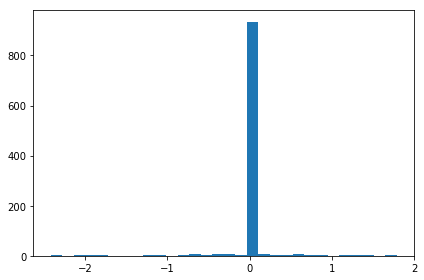
\includegraphics[width=0.24\pagewidth]{Figure01.png}
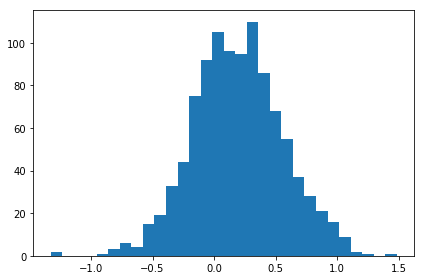
\includegraphics[width=0.24\pagewidth]{Figure02.png}
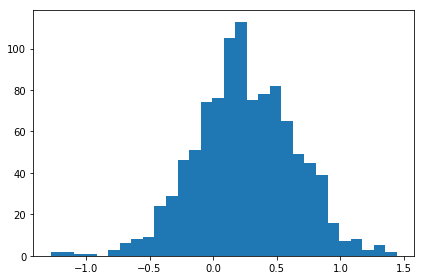
\includegraphics[width=0.24\pagewidth]{Figure03.png}
\caption{Histogram of solutions (Left: CVX-MOSEK, middle: Algorithm \ref{Alg:ProjNaive}, right: Algorithm \ref{Alg:SubNaive})} \label{Fig:SparseHist}
\end{figure}
To settle this issue, the regularization should be increased, and therefore an exponentially decreasing sequence of $\mu$ is introduced. Note that $ i_0 = 1500 $, and therefore the gradient method runs for 500 iterations for the original optimization problem, which ensures the solution not distorted.

Note that the Gurobi is not compatible with the memory model of Python, which results in a difficiency in setup time. To be exact, the Python version of Gurobi uses a class named \verb"tupledict" to handle matrices and tensors which cannot be directly converted to \verb"numpy.array", and therefore conversion accounts for the abnormal long setup time. The solve time makes sense anyway.

	\end{document}
